\documentclass{article}
\usepackage[utf8]{inputenc}

\title{Summary of Project Work During Student Internship}
\author{Keenan McConkey}
\date{December 2018}

% ****** TODO ******
% 0) Final edit
% 1) Ask Sascha about focused VEED beam image

% **** COMPLETE ****
% Look through MATLAB files for graphs to include
% Remove notes on 80 ms delay needed for REGAE
% Update Chopper 2 on delay
% Talk about updated VEED disk calculations
% Update timing diagram with better names, pre/post Ch2 in slippage diagram
% Add CAD drawing of calibration stage
% Write all Discussion subsections
% Check for consistent formatting of code w/ \texttt{}
% Include pictures taken in Munich
% Add Thorlabs documentationc
% Include IP Address check step (& Yaskawa login info)
% Update VEED diagram

\usepackage{graphicx}
\usepackage{enumitem}
\usepackage{natbib}
\usepackage{verbatim}
\usepackage{geometry}
\usepackage{url}
\usepackage{hyperref}

\geometry{textwidth=15cm}
\geometry{margin=1.0in}
\begin{document}

\begin{titlepage}
    \centering
    \Huge
    \textbf{Summary of Project Work During Student Internship}
    
    \vspace{1cm}
    \Large
    May 2018 to December 2018
    
    \vspace{2cm}

    \textbf{Keenan McConkey}
    
    \vfill
    
\includegraphics[scale=0.25]{img/ubc_logo}  
    \hspace{1cm}
    
\includegraphics[scale=0.5]{img/mpsd_logo}
    
    \vspace{3.5cm}
    Supervisor:
    
    \vspace{0.5cm}
    \textbf{Dr. Sascha Epp} 
\end{titlepage}

\tableofcontents
\listoffigures
\pagebreak

\section{Abstract} \label{abstract}

   The purpose of this report is to document work done on various projects during my undergraduate internship from May to October 2018.  This will include an overview of each of these projects, and an explanation of the approach used to complete them. It may also include discussion on the results and future of these projects. It is hoped that this document will serve as a clear reference for the continuation and maintenance of these projects by future student interns.

\section{Introduction} \label{introduction}

    The majority of project work was done under the supervision of Dr. Sascha Epp of the MPSD, as part of completing the co-op portion of my BASc. degree at the University of British Columbia, Engineering Physics faculty. Much of the work done on the \textbf{VEED/REGAE Chopper System} and \textbf{VEED Experimental Setup} was a collaboration with fellow student intern Pawel Mirksi.  Note that a large amount of progress on the \textbf{Chopper System} and the \textbf{BNC Server Arduino} was inherited from previous student interns Mohamed-Ali Hached and Saman Shariat Jaffari. For the purpose of comprehensiveness, there will be some overlap between our respective reports.
    
    The various projects detailed in this report include the use of Arduino microcontrollers, servo motors, programmable logic controllers, control theory, laser optics, CAD, amplifier design, interrupts, serial communication, and TCP/IP networking. Programming languages used include Arduino-C, Python, HTML, and IEC 61131-3. All applicable reference documentation is found in the appendix of this report.

\section{REGAE/VEED Chopper System} \label{chopper_system}

    \subsection{Overview} \label{overview}
    
        In certain beam line experiments, mechanical choppers are used to control the frequency and pulse length at which a beam hits a sample. In our case, this is done using a aluminum disk with a machined opening along its radius. While spinning at a constant RPM of 50 rev/s, the disk blocks an incoming beam at a controlled frequency. The dimensions of the disk's opening then control the time window during which the beam can pass through the chopper.
        
        In our setup, a secondary chopper is also placed in the beam line after the primary one. This chopper acts to "pick and choose" beam pulses outputted from the first chopper at sub-multiples of the frequency at which they leave the first. Unlike the first, this secondary chopper is not a disk. Rather, it is a machined cylinder with multiple holes along its radius. By switching between a blocked position and a position where a beam can pass through one of these holes, this chopper can select pulses when triggered by an input trigger signal.
        
        Since Chopper 2 takes some time to move from closed to open position, it always has to be triggered off a Trigger rising edge one edge before it actually needs to be open to allow the beam to pass. When triggered, it waits delays for a set time, determined to be 41.5 ms, before beginning its movement to the open position.
        
        For the rest of all documentation this primary and secondary chopper are referred to as \textbf{Chopper 1} and \textbf{Chopper 2} respectively.
        
        \begin{figure}[h]
            \centering
            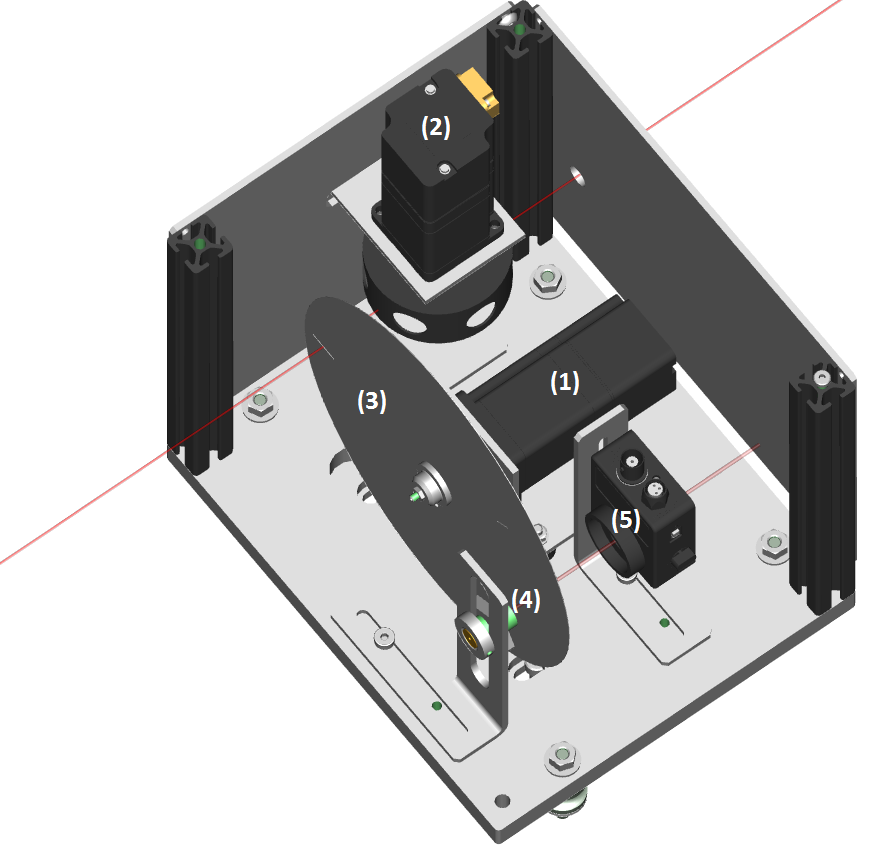
\includegraphics[width=11cm]{img/chopper_full_cad}
            \caption{CAD model of Chopper System: (1) Chopper 1; (2) Chopper 2; (3) Chopper 1 disk with two openings; (4) HeNe Laser; (5) HeNe Detector}
            \label{fig:chopper_full_cad}
        \end{figure}
    
        \subsubsection{Feedback HeNe Laser}
        
            An important component of this chopper system is the feedback HeNe laser. Since it is critical to know the time at which Chopper 1 will let a pulse pass through, a second opening has been machined into the disk of Chopper 1 with a continuous-wave HeNe laser aligned at its radius (Note that it is not actually a HeNe laser but is called so by convention). While the chopper spins, the HeNe hits a detector on the chopper's opposite side which converts the periodic chopping of the HeNe into a 50 Hz pulse signal, which we call the \textbf{HeNe Reference} signal. By the geometry of Chopper 1's disk, we know a HeNe Reference pulse will be generated 2 ms before the chopper is open to the beam (when spinning at 50 rev/s). Thus we precisely know when the beam will be able to pass through the chopper.
            
        \subsubsection{Yaskawa Motion Controllers}
        
            Each of Chopper 1 and Chopper 2 are controlled by two independent Yaskawa MP2600iec programmable logic controllers \cite{mp2600}, which are connected to Yaskawa Sigma-5 servo motors \cite{sigma5}. These controllers are intended for use in high-precision, high-speed servo motor applications, and include software that allows for programming of various movements. They also include connected digital and analog I/O ports. Similarly they can communicate via TCP/IP for configuration by a PC or for general client-server interactions. 
        
    \subsection{Delay Error Correction} \label{chopper_error}
    
        Knowing the time at which the beam can pass through the chopper is only useful if we can align it to another action. We use one square wave signal to align the timing of the whole system (simply called the \textbf{Trigger} or \textbf{12.5 Hz Trigger}). This trigger is generated independently of the choppers. 

        We use a Arduino Due to calculate timing error, which measures the time delay between the HeNe Reference pulse and the rising edge of the Trigger. The Arduino then converts this to a analog voltage which is read by the Yaskawa motor controller for Chopper 1 as a time delay. The motor controller continuously adjusts Chopper 1 so that this time delay is 2 ms, i.e. Chopper 1 open consistently at the rising edge of the Trigger (demonstrated in Figure \ref{fig:chopper_osc}).
        
        \begin{figure}[h]
            \centering
            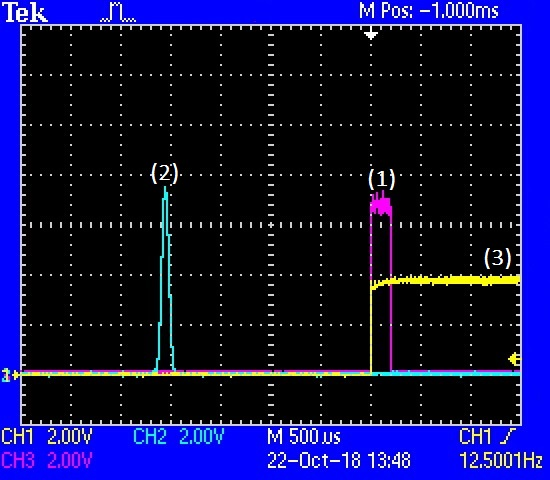
\includegraphics[width=8cm]{img/chopper_osc}
            \caption{Oscilloscope view of Chopper System: (1) Pulse passing through the chopper; (2) HeNe Reference; (3) 12.5 Hz Trigger rising edge}
            \label{fig:chopper_osc}
        \end{figure}
        
        If Chopper 1 becomes unaligned so that this delay is not 2 ms, Chopper 1 corrects by spinning at slightly higher or lower velocity until the its open position aligns again with the rising edge of the Trigger. The velocity profile is shown in Figure \ref{fig:chopper_vel_profile}. By integrating the area under this Velocity-Time curve, one can calculate the position correction obtained by executing this velocity shift. Formulas were determined for calculating $\Delta v$ and $t_1$. 
        
        \begin{figure}
            \centering
            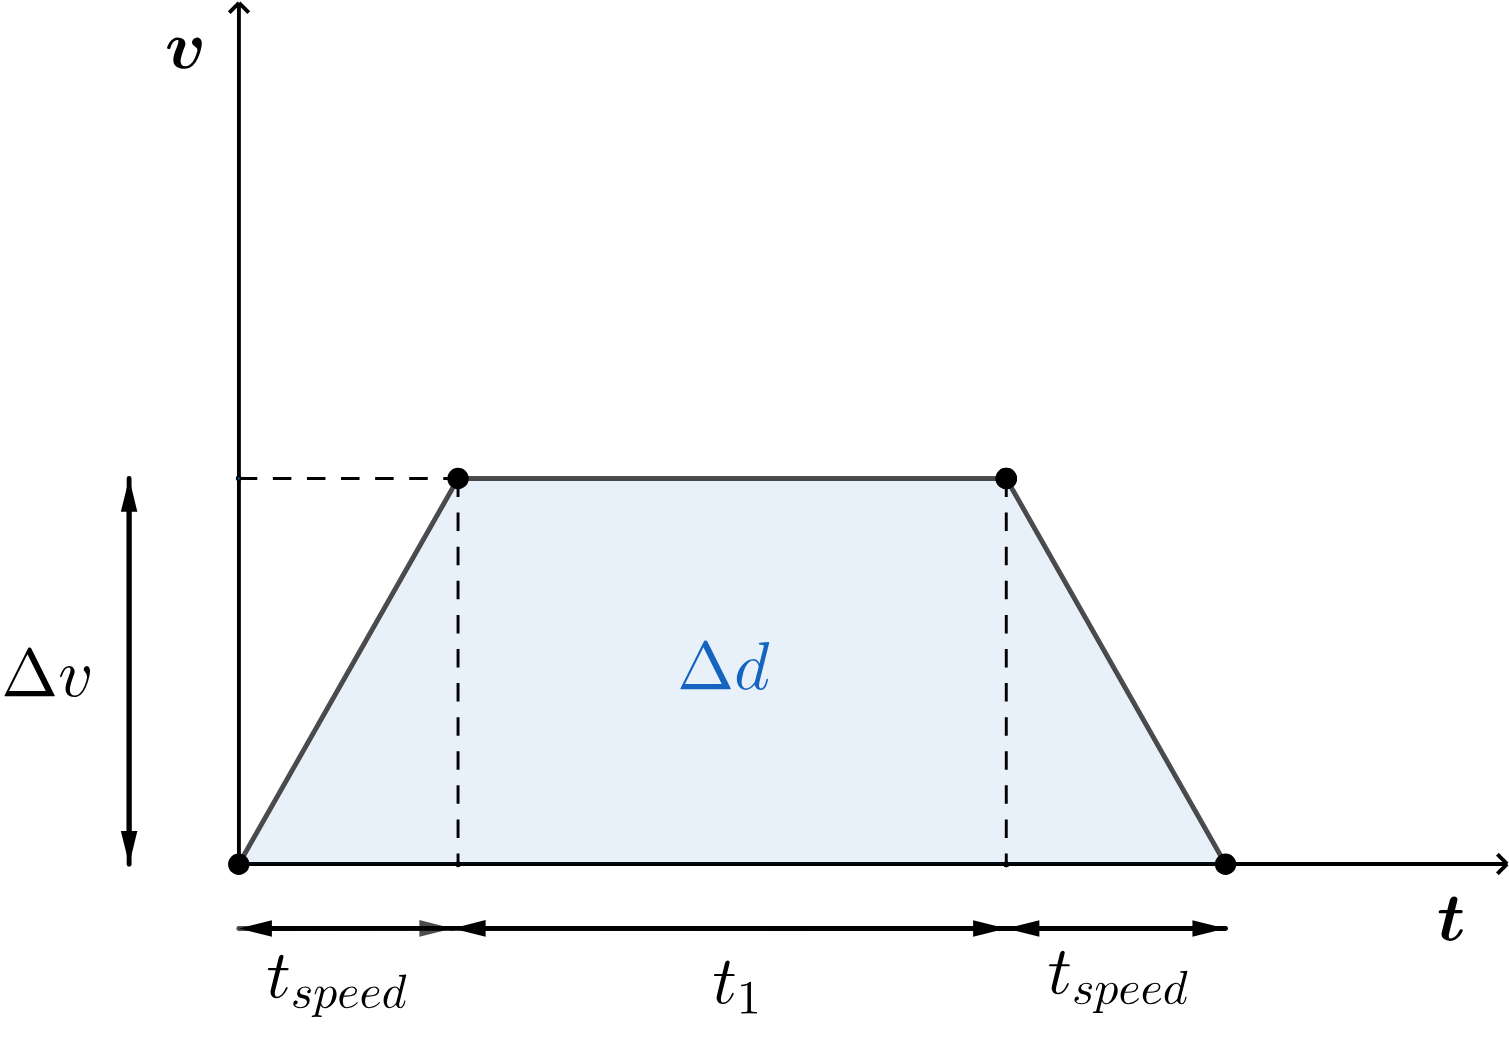
\includegraphics[width=8cm]{img/chopper_vel_profile}
            \caption{Velocity profile of Chopper 1 correction}
            \label{fig:chopper_vel_profile}
        \end{figure}
        
        \begin{equation}
            t_1 = \frac{t_{speed}}{2} + \sqrt{\frac{t_{speed}^2}{4} + \frac{|\Delta t|}{T_{rev}\cdot a}}
        \end{equation}
        
        \begin{equation}
            \Delta v = a \cdot t_1
        \end{equation}
        
        Where...
        
        \begin{itemize}
            \item $t_{speed} = $ Time it takes for Chopper 1 to accelerate to new velocity, constant (36 ms)
            \item $\Delta t = $ Time error calculated by Arduino (deviance from 2 ms)
            \item $T_{rev} \ = $ Period of one revolution of Chopper 1 at 50 rev/s (20 ms)
            \item $a = $ Acceleration of Chopper 1, constant
        \end{itemize}
        
        Since the velocity of the disk is not precisely 50 rev/s at all times (a property of servo motors), some error in time delay between HeNe Reference, and therefore open hole position, and 12.5 Hz Trigger rising edge will always accumulate over time. Thus this correction routine must be performed continuously as Chopper 1 runs.
    
    \subsection{REGAE vs VEED} \label{chopper_regae_veed}
    
    The Chopper System is intended to be used in two separate beam line setups at the institute:
    
    \begin{itemize}
        \item \textbf{REGAE} - Relativistic Electron Gun for Atomic Exploration
        \item \textbf{VEED} - Virtual Electron Daemon
    \end{itemize}
    
    In both of these setups,  Chopper 1 is to spin at a constant speed of 50 rev/s, which fixes the frequency of beam pulses exiting it at 50 Hz (or once every 20 ms). Chopper 2 is free to be configured at any sub multiple of Chopper 1's frequency as set by the Trigger signal.
    
    %Both of the beam lines have a common source of error accumulation. Unlike the chopper systems, the beam lines are not powered off of main line AC power. Since the frequency (approximately 50 Hz in Germany) of main line power constantly fluctuates a small amount, a time delay error always accumulates between the HeNe Reference pulse and the rising edge of the Trigger (which is generated by the beam line). Therefore the delay correction routine must constantly correct for this error accumulation as well.
    
    \subsubsection{REGAE}
    
        In the \textbf{REGAE} application, a pulsed laser beam (sometimes called the \textbf{P-Laser} or \textbf{Main Laser}) with a pulse length of approximately 100 femtoseconds is to hit the dual choppers at a frequency of 1 kHz.  Chopper 1 spinning at 50 rev/s allows 1 out of every 20 of these 1 kHz pulses to pass, and Chopper 2 then further chooses 1 out of 4 of these pulses, resulting in pulses output at a frequency of 12.5 Hz. In this is experiment, we want the Main Laser to hit a sample at the exact same time as a pulsed electron beam. The Trigger in this case is generated by that electron beam, with equivalent phase.
        
        \begin{figure}
            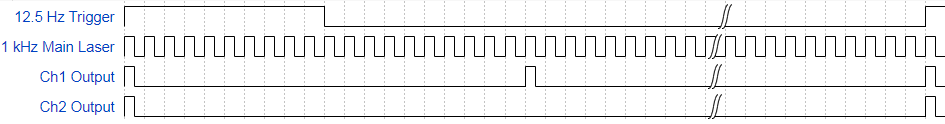
\includegraphics[width=1.0\textwidth]{img/regae_timing}
            \caption{Timing diagram for REGAE}
            \label{fig:regae_timing}
        \end{figure}
        
        An important condition of this setup is the "slippage" of the Trigger. All AC wall power electrical lines maintain some frequency (in Germany this is 50 Hz), but due to fluctuations in customer usage this frequency is not constant. This causes an accumulation in phase error between the Main Laser generated by wall power and the Trigger which is generated independently. Therefore after the system runs for some time the Trigger will suddenly slip out of phase with the Main Laser, such that the Trigger is now aligned with a Main Laser pulse one pulse earlier than before. This is pictured in Figure \ref{fig:regae_slippage}.
        
        \begin{figure}[h]
            \centering
            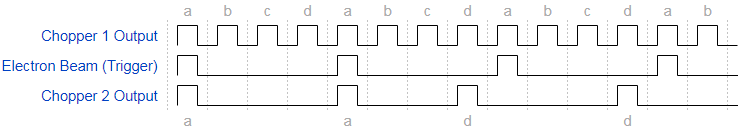
\includegraphics[width=12.5cm]{img/regae_slippage}
            \caption{REGAE slippage condition}
            \label{fig:regae_slippage}
        \end{figure}
        
        When this slippage condition occurs, the time delay between HeNe and Trigger rising edge suddenly becomes very high. Chopper 1 must be able to correct for this sudden change as quickly as possible to avoid misaligned pulses hitting the sample. Currently, this correction time takes approximately 160 ms.
    
    \subsubsection{VEED}
    
        In the \textbf{VEED} application, a continuous laser beam is to be chopped into pulses by the system. Again Chopper 1 is fixed at 50 rev/s, and Chopper 2 chooses pulses output from Chopper 1 to allow through. However, in the VEED case Chopper 2 can theoretically select any integer sub-multiple of 50 Hz to output, i.e. 12.5 Hz, 25 Hz or 50 Hz. A new disk for Chopper 1 was designed with a small opening slit (width 1 mm) to generate short pulses from the input continuous beam. In this experiment, the Trigger is only used for synchronization of the system, which we create with a function generator.
        
        \begin{figure}[h]
            \centering
            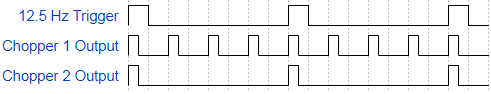
\includegraphics[width=8.5cm]{img/veed_timing}
            \caption{Timing diagram for VEED}
            \label{fig:veed_timing}
        \end{figure}
        
        As the beam input to the system is continuous, we don't need to worry about slippage from the trigger. Constant correction of Chopper 1 is still needed because of the previously mentioned condition of non-constant disk velocity.
    
    \subsection{Implementation} \label{chopper_implementation}
    
        \subsubsection{Motionworks}
        
            The Yaskawa motion controllers use a custom programming environment called Motionworks IEC. It already include libraries for motor control routines. It also allows for the creation of SFCs (Sequential Function Charts) which makes implementing the logic of motion control easier. Yaskawa has created a series of YouTube videos \cite{motionworks_youtube} as an introduction to their programming environment. Additional documentation \cite{motionworks} is always useful.
            
        \subsubsection{Ethernet Control}
        
            \begin{figure}[h]
                \centering
                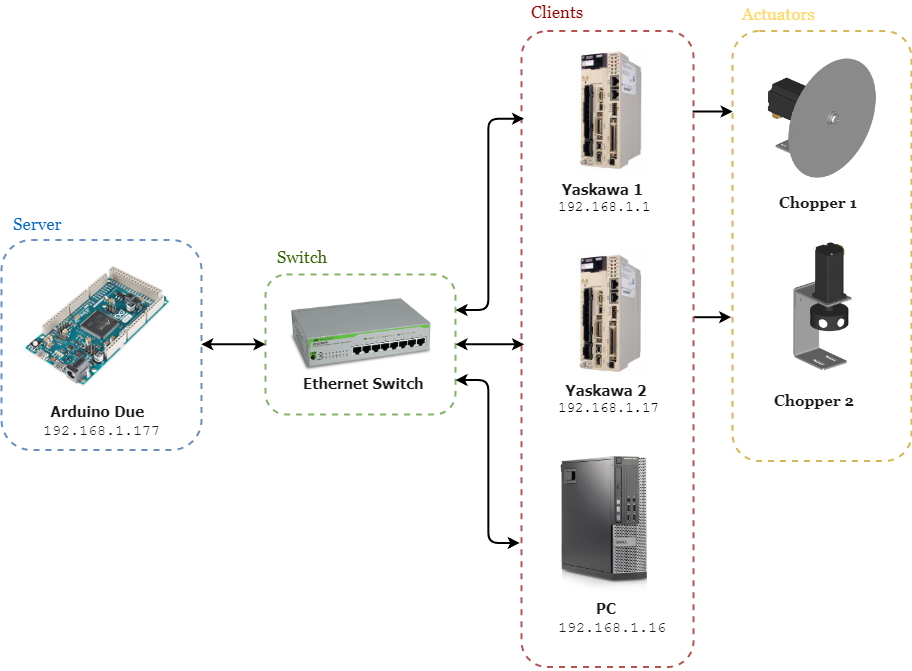
\includegraphics[width=13cm]{img/regaedat_lan}
                \caption{LAN for Ethernet control of Chopper System}
                \label{fig:regaedat_lan}
            \end{figure}
            
            One of my main contributions to the Chopper System during my stay was the creation of a network of devices to control the system. The central device of this network is the \textbf{BNC Server Arduino}, which acts as a server to accept client connections over Ethernet (on top of performing the delay error calculations above).
            
            With this Arduino acting as a server, a PC on the local network can connect as a client and send commands to be executed by the chopper system. This is implemented in the form of a \texttt{HTML} website hosted by the Arduino, which allows a PC user to enter information to be transmitted as an \texttt{HTTP Query}. \texttt{Javascript} is then used to verify user data. When a new command is sent, the website updates to reflect the change.
        
            \begin{figure}[h]
                \centering
                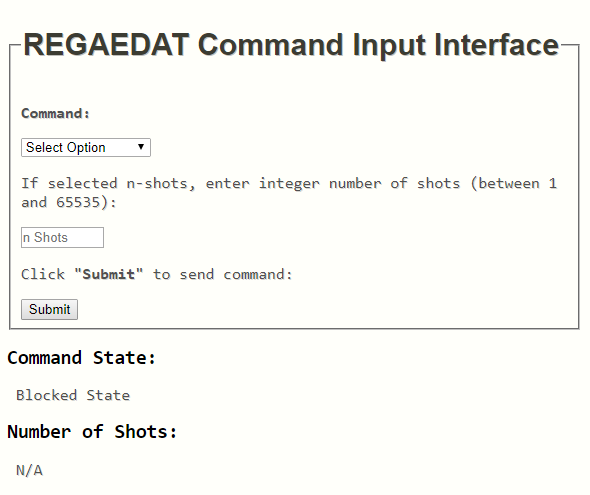
\includegraphics[scale=0.65]{img/command_interface}
                \caption{HTML Command interface hosted by the Server Arduino}
                \label{fig:command_interface}
            \end{figure}
            
            The Yaskawa motion controllers are also able to connect to the Arduino server as a client. When a command is received by the Arduino from a PC, the Arduino stores this command locally. A Yaskawa controller is then able to connect to the Arduino at regular intervals and update itself on a change in command from the PC, which changes the functionality of the choppers. The control loop implementation of client behaviour is shown in Figure \ref{fig:ethernet_sfc}.
            
            A custom transmit/receive buffer had to be created for the choppers and Arduino to send/receive data on the network. To minimize transmission delay, it was decided that the optimal buffer size would be \texttt{16-bytes}. Yaskawa 1 and 2 and the Arduino all read/write predefined \texttt{char} to the buffer to represent different actions. The configuration of bytes Yaskawa 1 and 2 send/receive with the Arduino over these buffers is as follows:
            
            \begin{quote}
                \centering
                \texttt{[0|1|2|3|4|...|15]}
            \end{quote}
            
            \textbf{Yaskawa 1:}
            \begin{itemize}
                \item [\texttt{0}]: Must be '$>$' character (ASCII 62). Similar to '?' in HTTP
                \item [\texttt{2}]: Value of Command State for Yaskawa 1 (0 to 255)
            \end{itemize}
            
            \textbf{Yaskawa 2:}
            \begin{itemize}
                \item [\texttt{0}]: Must be '$<$' character (ASCII 60). Similar to '?' in HTTP
                \item [\texttt{2}]: Value of Command State for Yaskawa 2 (0 to 255)
                \item [\texttt{4}]: Least significant byte of n Shots data (0 to 65535)
                \item [\texttt{5}]: Most significant byte of n Shots data
                \item [\texttt{7}]: Protocol bit for transmission control (1 or 0)
                \item [\texttt{9}]: Value of Command State for Y1 to send/receive (0 to 255)
            \end{itemize}
            
        \subsubsection{Chopper 1}
        
            Most of functionality of Chopper 1 had already been implemented by previous interns. However, a loss of data meant parts of the code had to be rewritten. We also worked on adding Ethernet communication functionality to both choppers. Chopper 1 code was modified to be in the SFC form shown in Figure \ref{fig:ch1_sfc} (Appendix). The current implementation of Chopper 1 allows for four different commands to be executed:
            
            \begin{itemize}
                \item \textbf{Stop} - Stop all movement of the chopper
                \item \textbf{Spin} - Run regular chopping functionality
                \item \textbf{Open} - Align the chopper hole to allow the beam to pass
                \item \textbf{Close} - Align the chopper hole to block the beam
            \end{itemize}
            
            \noindent Chopper 1 receives an update on its command state from the Arduino, but for timing purposes, Chopper 2 controls when the Arduino changes its locally stored command state for Chopper 1, i.e. we cannot directly send commands to Chopper 1. Chopper 1 essentially acts as the slave in a Master-Slave relationship with Chopper 2.
            
        \subsubsection{Chopper 2}
        
            Chopper 2 functionality was greatly expanded. A number of commands needed to be implemented for use in the different setups, including:
            
            \begin{itemize}
                \item \textbf{Block} - Align the chopper hole to block the beam
                \item \textbf{Continuous Wave} - Align the chopper hole to allow the beam to pass
                \item \textbf{Single Shot} - Allow a single beam  pulse to pass through the chopper
                \item \textbf{N Shots} - Allow $n$ number of beam pulses to pass through the chopper
                \item \textbf{Continuous Shots} - Allow beam pulses to pass until stopped
            \end{itemize}
            
            \noindent The execution of these different commands is done using an SFC control loop, shown in Figure \ref{fig:ch2_sfc} (Appendix). Chopper 2 functionality is completely determined by what is input into the HTML interface and can function without Chopper 1.
            
        \subsubsection{System Housing}
        
            Work was done during my stay to reduce the size of the Chopper System's footprint. Chopper 2 was adapted to fit directly inside the housing originally only used for Chopper 1. Pieces were reused in conjunction with newly manufactured parts to minimize the size of the system while still providing a safe housing. Overall, a 46\% reduction in system footprint area was achieved, without including the area reduction from moving Chopper 2 into the housing.
            
    \subsection{Discussion}
    
    In its current state, the Chopper System was used effectively for experiments in the VEED application. Possible areas of improvements in the system include: reducing overall delays in the system, including Chopper 1 velocity correction delays and Chopper 1/2 startup delays; optimizing and testing Chopper 2 to work with frequencies other than 12.5 Hz; creating verification tool that checks that an "N Shots" command sends the correct number of shots; and improving overall error-handling in the system.
    
\section{VEED Experimental Setup} \label{veed_setup}
    
    \subsection{Overview} \label{veed_setup_overview}
    
    \begin{figure}[h]
        \centering
        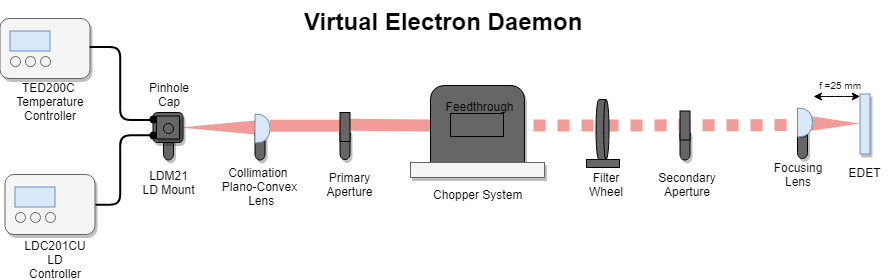
\includegraphics[width=1.0\textwidth]{img/veed_schematic}
        \caption{Schematic of VEED}
        \label{fig:veed_schematic}
    \end{figure}
            
    VEED is a beam line daemon created to simulate a pulsed electron beam using packets of photons with equivalent energy. This is to be used for calibration and debugging of an \textbf{EDet} (Electron Detector) sample, in this case a high-speed detector for use in imaging applications. Energy equality of $n$ photons equal to one electron can be calculated at a given wavelength:
    
    \begin{equation}
        E_{e^-} = n \cdot E_{\gamma} = n \cdot \frac{hc}{\lambda}
    \end{equation}
    
    Where...
    \begin{itemize}
        \item $h = $ Planck's constant 
        \item $c = $ Speed of light
        \item $\lambda = $ Wavelength of the photons
    \end{itemize}
    
    \noindent In order to reach an energy comparable to singular electrons an 880 nanometer laser has to be greatly reduced in optical power. Note that since optical power and number of photons per second are proportional we can think of them interchangeably.
    
    \subsubsection{Chopping}
    
     As previously described, the input to the VEED is a continuous wave laser beam, which is chopped into small pulses by the Chopper System. One can calculate the power of a single pulse output from the system using the geometry of Chopper 1 and both Chopper 1 and 2's chopping frequency.
    
    \begin{equation}
        P_{out} = \frac{P_{in}}{v_1 v_2} \cdot \frac{d_{slit}}{2\pi r_{slit}}
    \end{equation}
    
    Where...
    \begin{itemize}
        \item $P_{in} = $ Optical power of the input continuous-wave beam
        \item $v_1, v_2 = $ Speed of Choppers 1 and 2, respectively, in revolutions per second
        \item $d_{slit} = $ Width of machined slit in disk of Chopper 1
        \item $r_{slit} = $ Radius of machined slit, assumed large compared to width
    \end{itemize}
    
    \subsubsection{Filtering}
    
    Beam power is further reduced by filtering to get down to power equivalence of an electron. We use neutral density (ND) filters to greatly reduce beam power. An ND filter is characterized by its optical density, which reduces the power of the beam exponentially:
    
    \begin{equation}
        \frac{I}{I_0} = \frac{P}{P_0} = 10^{-d}
    \end{equation}
    
    Where...
    \begin{itemize}
        \item $I_0 \ = $ Incident beam intensity
        \item $P_0 = $ Incident beam power
        \item $d \ \ = $ Optical density of the filter
    \end{itemize}
    
    \subsubsection{Beam Collimation}
    
    To be used in the relatively long distances of our setup, the input beam needs to be collimated. A perfectly collimated beam of light has parallel rays, such that it does not diverge as it propagates. Perfect collimation is impossible due to diffraction, but we still try to minimize divergence as much as possible using lenses (e.g. 40 mm plano-convex lens).
    
    \begin{figure}[h]
        \centering
        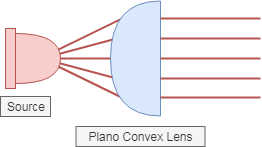
\includegraphics[scale=0.5]{img/collimation}
        \caption{Collimation with a plano-convex lens}
        \label{fig:collimation}
    \end{figure}
    
    \subsubsection{Diffraction}
    
    As shown in Figure \ref{fig:veed_schematic}, apertures are used in the setup to reduce beam diameter. However, at the low diameter apertures we use, diffraction becomes an issue as the wavelength becomes comparable to the aperture size. Thus various sized apertures are used to cut off diffracted beam patterns at multiple points along the setup.
    
    \subsubsection{Focusing}
    
    After finally reaching the desired beam power and thus the desired number of photons per second, the beam is focused in order to hit a single pixel of the detector. A beam diameter of approximately 100 micrometers was found to be effective for this goal.
    
    \begin{figure}[h]
        \centering
        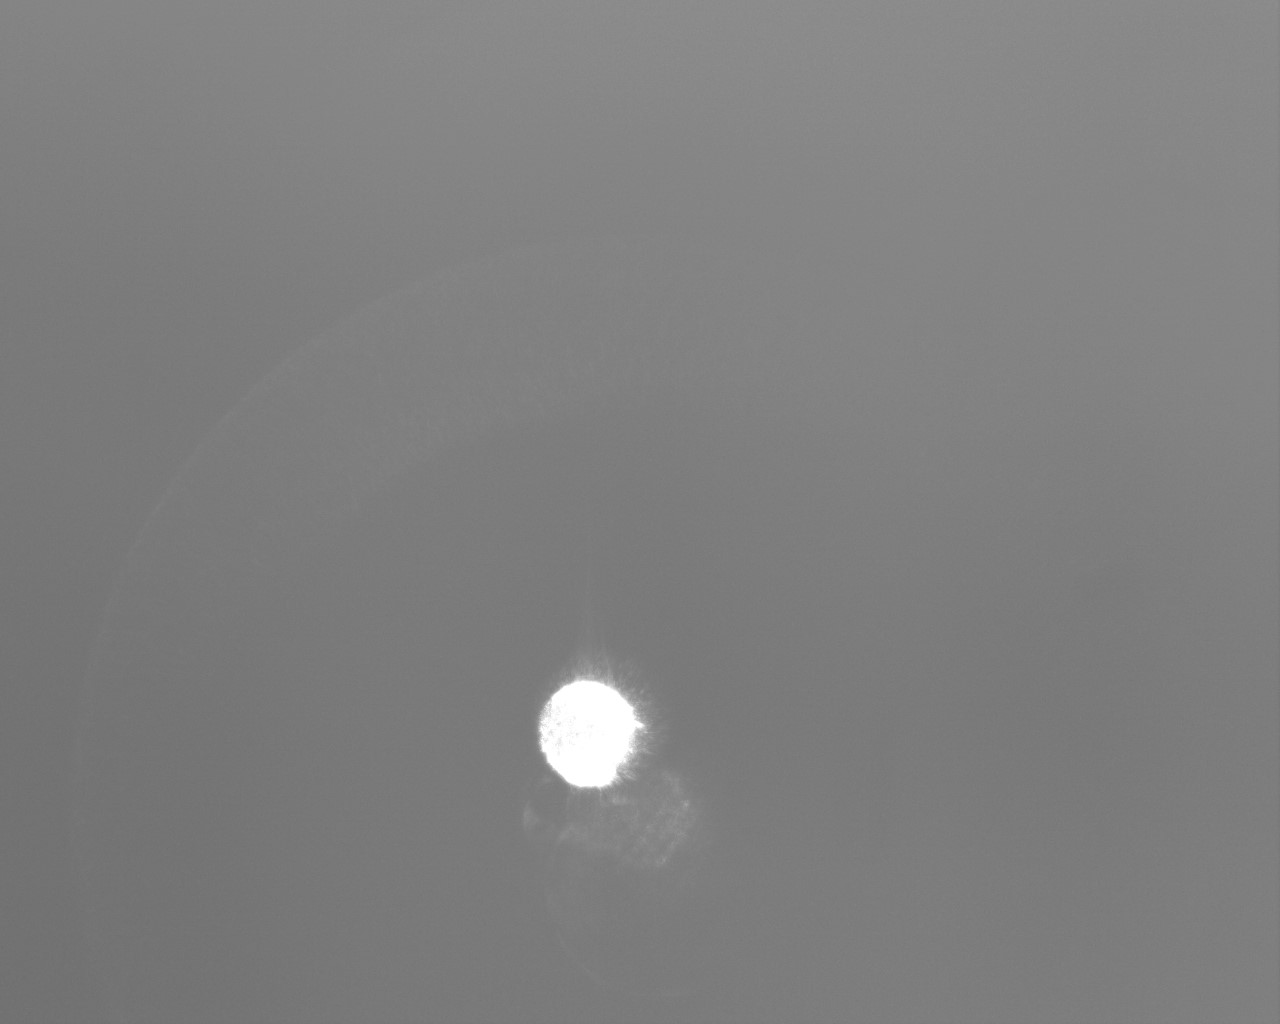
\includegraphics[scale=0.2]{img/15ma_beam}
        \caption{Unfocused VEED beam capture taken before Chopper System}
        \label{fig:15mA_beam}
    \end{figure}
    
    \subsection{Pinhole Power Cap} \label{veed_cap}
    
    A laser cap needed to be designed to ensure the beam power does not exceed the Class 1 laser limit of 1 mW at normal operating current. This cap had to fit on a purchased laser diode mount (LDM21) \cite{ldm21}. Optical power was measured at varying current inputs to the diode mount, and an optimal current for power close to 1 mW was determined (Figure \ref{fig:cap_power_plot}).
    
    \begin{figure}[h]
        \centering
        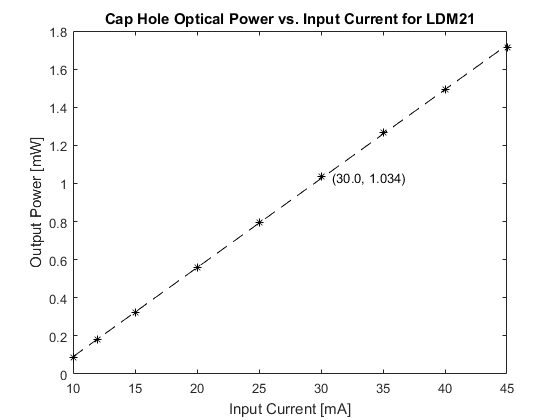
\includegraphics[scale = 0.6]{img/cap_power_plot}
        \caption{Optical power of capped laser}
        \label{fig:cap_power_plot}
    \end{figure}
    
    Special cap-screws were used to make it difficult for inexperienced users to remove the cap, and the cap was anodized in matte-black to minimize all back-reflections of the beam. In order to ensure we could change the size of the pinhole fairly easily, the cap was split into a pinhole piece and a mount, so that new pinhole pieces could be manufactured without having to remake the entire part.
    
    \begin{figure}[h]
        \centering
        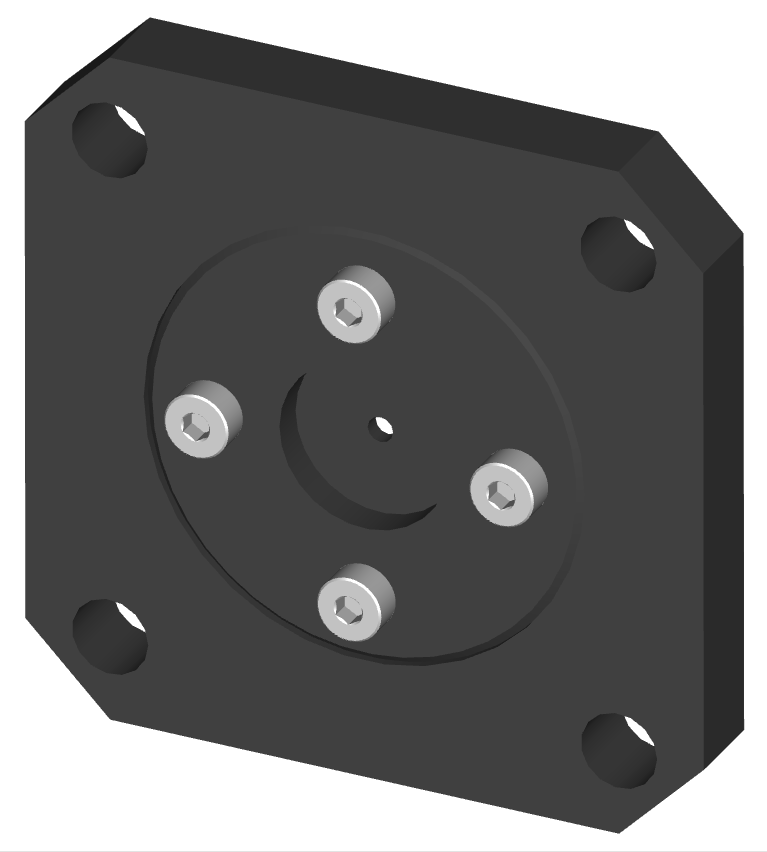
\includegraphics[scale = 0.2]{img/laser_cap_cad}
        \caption{Rear view CAD model of Laser Cap}
        \label{fig:laser_cap_cad}
    \end{figure}
    
    \subsection{Feedthrough Wall} \label{veed_wall}
    
    In order to minimize the effects of any stray photons on the sample, the VEED apparatus needs to be enclosed in a light-tight environment. This results in some difficulties in providing the necessary cables for the system. For general cables, a premade cable enclosure was purchased that allows for the insertion of variously sized cables while still keeping the VEED enclosure sealed.
    
    One of the cables for the EDet sample could not be fit into the premade part, so a custom feedthrough panel was designed to enable the insertion of this cable without compromising light sealing. This panel allows for rotation of the cable by $90^\circ$, and has adjustable clamps to hold the cable tightly.
    
    \begin{figure}[h]
        \centering
        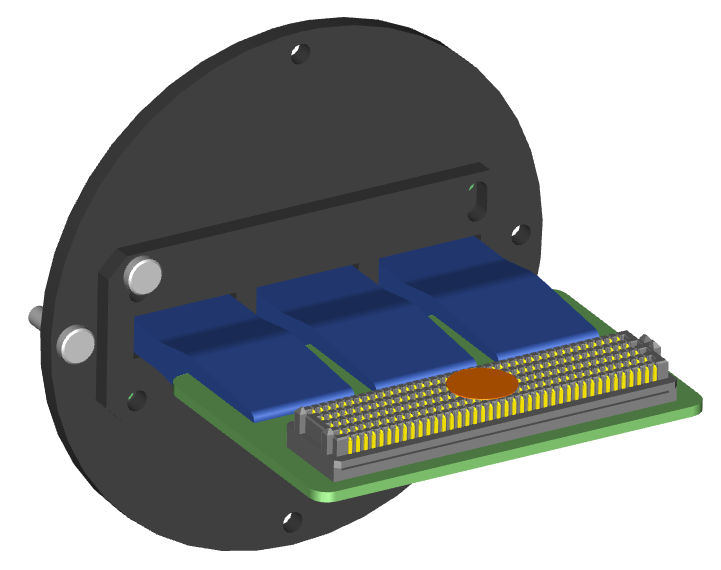
\includegraphics[scale=0.3]{img/feedthrough_panel_cad}
        \caption{CAD model of feedthrough panel}
        \label{fig:feedthrough_panel_cad}
    \end{figure}
    
    \subsection{Detector Stage}
    
    A liear 3-axis stage needed to be designed to facilitate movement of the beam to different pixels of the grid of pixels making up the detector. The detector also has to move into the 25 mm focal length of the beam. A custom mounting plate was machined for this purpose. In the future this could be motorized but currently the stages can only be moved manually.
    
    \begin{figure}[h]
        \centering
        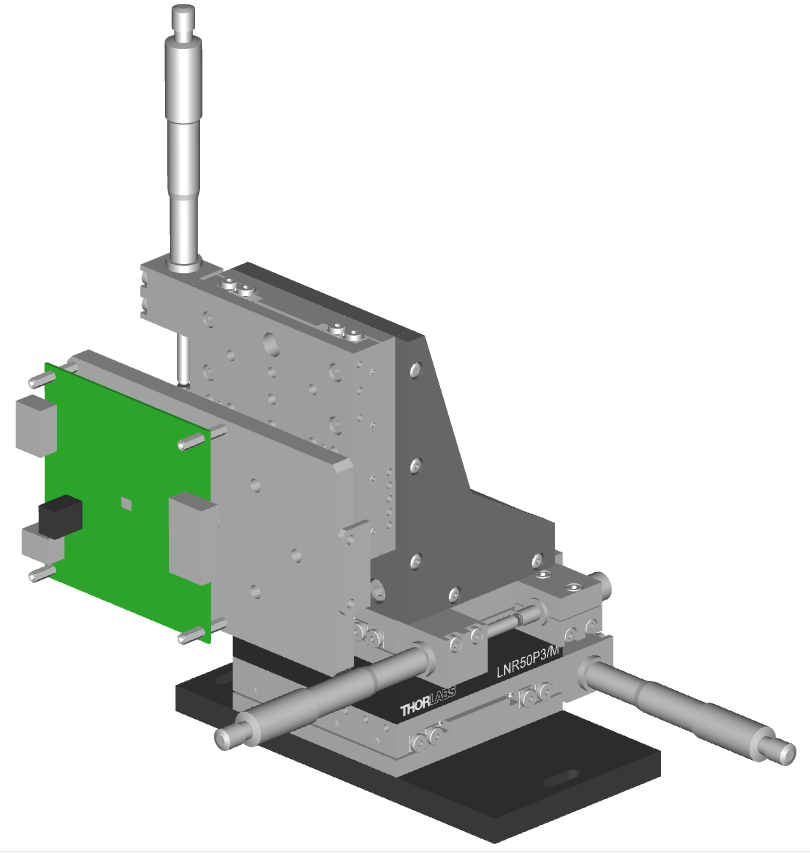
\includegraphics[scale=0.4]{img/calibration_cad}
        \caption{CAD of detector on the detector stage}
        \label{fig:calibration_cad}
    \end{figure}
    
    \subsection{Discussion}
    
    The VEED system has shown potential as a calibration device for electron detectors. The setup was taken to the Max Planck HLL detector lab in Munich for testing. There we produced illumination of a single detector pixel, which is crucial component detector calibration. As described, the detector can be manually moved using the stage for probing of different detector pixels. Different probing modes can be selected using the Chopper System HTML interface. Unfortunately, I do not have access to the electron detector data and thus cannot include relevant graphics showing pixel detection.
    
    \begin{figure}[h]
        \centering
        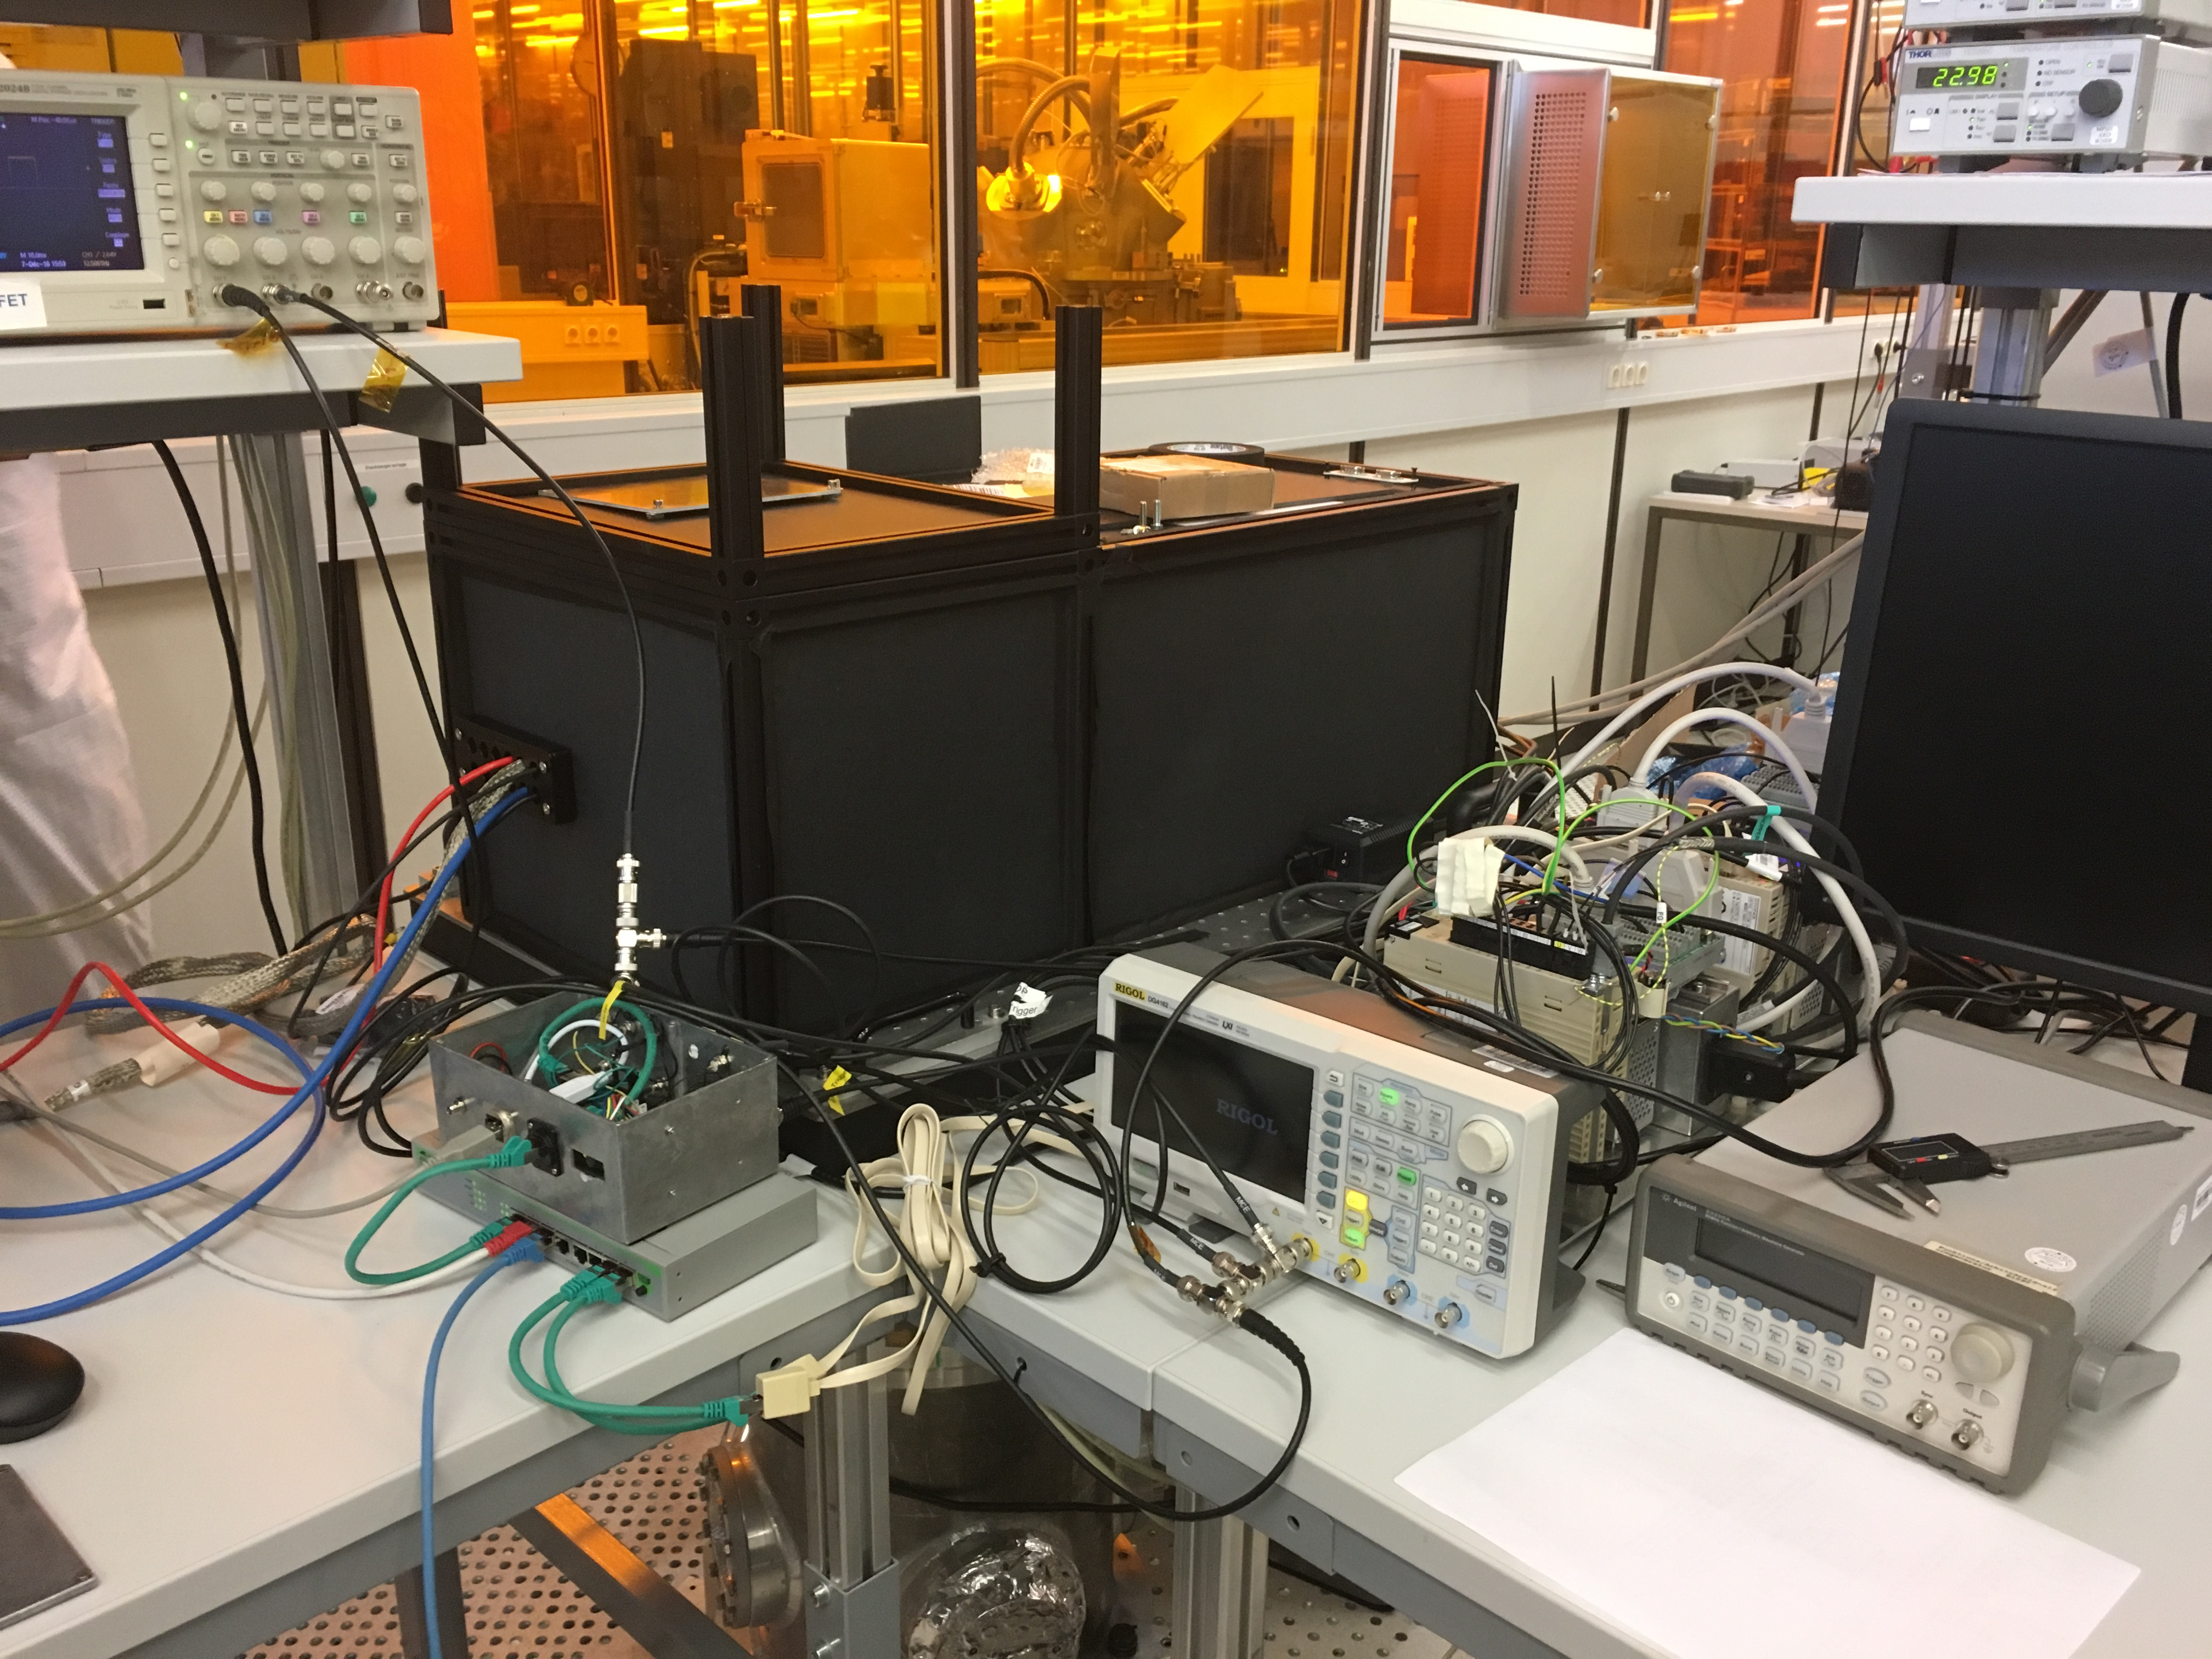
\includegraphics[width=0.75\textwidth]{img/munich_setup}
        \caption{VEED setup in MPG HLL Munich}
        \label{fig:veed_setup}
    \end{figure}
    
    The obvious area of improvement of this project is the motorization of the detector stage. After this is completed, the detector's movement could be synchronized with the software of the detector for automated calibration of every pixel.
    
    \section{BNC Server Arduino} \label{arduino}
    
        \subsection{Overview} \label{arduino_overview}
        
        An Arduino Due has been used to implement a variety of different functions simultaneously, as needed for the Chopper System. These include
        
        \begin{itemize}
            \item Acting as an Ethernet server with connected SD card memory
            \item Communicating with other devices over USB and RS232 serial
            \item Measuring the time delay between two input pulse signals (\textbf{VTT})
            \item Counting number of pulses over time on an chosen input signals
        \end{itemize}
        
        Implementation of time delay and USB/RS232 serial communication functionality was completed by previous interns, however work was done to greatly expand the number of commands executable over serial. These commands can be used to debug all of the different functions of the Arduino over a PC connection via USB. At present, the commands available over serial are as follows:
        
        \begin{verbatim}
    Basic Commands:
    * ? - Returns info on the system
    * help - Returns a list and info on commands
    * server:? - Returns info on server settings
    SD Card Commands:
    * sd:? - Get information about the SD card
    * sd:print - Get the contents of the SD card root directory
    * sd:printFile:[file] - Print the contents of a file
    * sd:remove:[file] - Remove a file from the root directory
    VTT Commands:
    * vtt:? - Get the current config of VTT
    * vtt:[d_in1]:[d_in2]:[a_out] - Set the BNC input/outputs
    * vtt:[time(us)] - Set the maximum delay time
    * vtt:start:2CHAN - Start 2 channel function
    * vtt:stop - Stop VTT function
    Yaskawa Commands:
    * yaskawa:? - Get current command state and n shots
    * yaskawa:state:[0-255] - Change Yaskawa state
    * yaskawa:nShots:[0-65535] - Change Yaskawa n shots
    CountPulses Commands
    * countPulses:? - Get CountPulses config
    * countPulses:command - Print all CountPulses commands
        \end{verbatim}
        
        \subsection{Ethernet Server} \label{arduino_server}
        
        By attaching an Ethernet Shield, the Arduino can act as an Ethernet server that accepts client connections from both PCs and Yaskawa motion controllers. When connected to by a PC,the Arduino hosts a web interface which the PC can then use to send commands back to the Arduino. The Arduino stores these commands in local variables, which the Yaskawa controllers can then access by connecting to the Arduino themselves. Put together, this allows a user to control the Yaskawa controllers remotely from any PC using a straightforward web interface. 
        
        Website HTML code is stored on a SD card connected to the Arduino. This implementation uses the native Arduino libraries \texttt{Ethernet} \cite{ethernet_library} and \texttt{ESP8266 SD} \cite{sd_library}, which are well-documented. Communication protocol is further detailed in Section \ref{chopper_implementation}.
        
        \subsection{Time-to-Voltage Converter} \label{arduino_vtt}
        
        The Arduino measures the time delay between two digital input signals through the use of interrupts. When a rising edge is detected on Digital Input 1, ISR 1 starts a time counter. The Arduino then waits until a second rising edge is detected on Digital Input 2, at which point ISR 2 resets the counter and writes it to Analog Output (which has a built in DAC). If a rising edge detected on Digital Input 1 before Digital Input 2, the counter is reset and the value output on Analog Output is not changed.
        
        Analog output on the Arduino Due has a resolution of \texttt{12-bits}, so the time value is converted to a value between 0 and $2^{12}=4096$. Thus a maximum time delay is needs to be set at 4095. When delay goes over this maximum, its value resets to 0. Details on the use of interrupts in Arduino Due can be found in the documentation of its Atmel 32-bit microcontroller \cite{atmel_sam3x_series} on board the Arduino. 
        
        In the chopper implementation, \texttt{Digital Input 1} is the HeNe Reference, \texttt{Digital Input 2} is the 12.5 Hz Trigger, and \texttt{Analog Output} is input into Yaskawas 1 and 2. This voltage was calibrated on the side of the Yaskawas, by graphing varying delay and calculating the linear relationship between delay and voltage measured at the Yaskawa analog input, shown in Figure \ref{fig:arduino-yaskawa_calibration}.
        
        \begin{figure}[h]
            \centering
            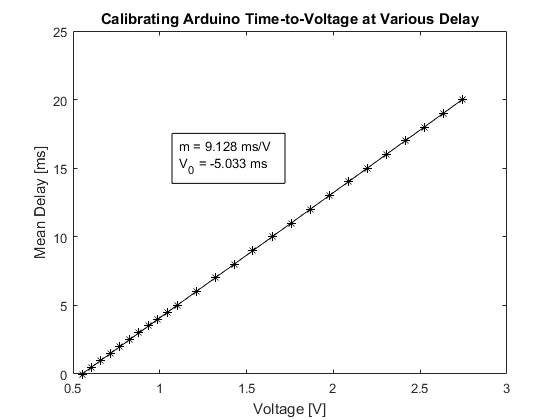
\includegraphics[scale=0.6]{img/arduino-yaskawa_calibration}
            \caption{Yaskawa-side voltage for varying delay input into Arduino}
            \label{fig:arduino-yaskawa_calibration}
        \end{figure}
        
        \subsection{Pulse Counter} \label{arduino_pulses}
        
        The Arduino is able to count the number of pulses (i.e. the number of rising edges) detected on a chosen \texttt{Digital Input}. An \texttt{ISR} is run to increment a counter every time a new pulse is detected. We can use this to verify that the number of shots output by the chopper system is correct by using a photodiode as the input.
        
        \subsection{Discussion}
        
        Overall, the BNC Server Arduino has been proven effective in multiple its multiple pre-described applications, including the VEED experiment. At present, no new features seem to be required, but testing and error-checking of the device are always helpful.
        
        
\section{Nanosecond Pulsing of an LED} \label{nanosecond_circuit}

    \subsection{Overview} \label{nanosecond_overview}
    
    To illuminate a sample for plume imaging during ablation experiments, a pulsed light source was needed with a pulse length on the order of nanoseconds and a repetition rate below 100 Hz. It was determined that an LED could be used for this application but a high-speed amplifier would be needed to boost input currents and voltage at high frequencies. The use of LEDs at nanosecond pulse-lengths is based on the work of Rose et al \cite{nanosecond_led}. High-speed amplifiers designs suitable for this purpose was found in Texas Instriuments' guide \cite{high_speed_amps}.
    
    \subsection{Implementation} \label{nanosecond_implementation}
    
    This project is currently at the breadboard prototyping stage. A circuit (see Figure \ref{fig:nanosecond_led_circuit}) was designed combining the circuits found in \cite{nanosecond_led} and \cite{high_speed_amps}. Certain resistors have been modified/removed to tune for the best possible amplification. An ultrahigh speed operation amplifier \cite{ad8009}, which performs at speeds up to 1 GHz, was purchased for use in the circuit.
    
    Amplification has been demonstrated with both nanosecond scale pulses (with varying repetition rates), and nanosecond period sine and square waves. Pulse length and input amplitude were found to have a significant effect on both the pulse length and a amplifier gain. Above 50 MHz pulse repetition rate the gain starts to decrease. 
    
    An oscilloscope probe was used to measure the voltage drop across the diode, as shown in Figures \ref{fig:pulse_amplfication} and \ref{fig:wave_amplification}. Amplifier gains of over 10dB were demonstrated. There was some difficulty with observing the LED light up at low pulse lengths, suggesting that the red LED\cite{cree_xpe_led} we chose may not be optimal for the nanosecond scale.
    
    \begin{figure}[h]
        \centering
        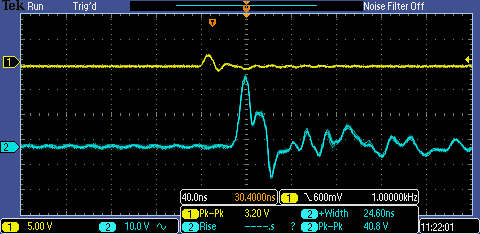
\includegraphics[scale=0.5]{img/pulse_amplification}
        \caption{Nanosecond-scale amplification of a 8 ns pulse}
        \label{fig:pulse_amplfication}
    \end{figure}
    
    \begin{figure}[h]
        \centering
        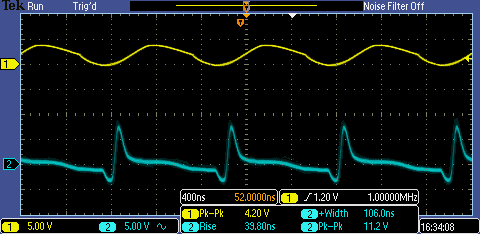
\includegraphics[scale=0.5]{img/wave_amplification}
        \caption{Nanosecond-scale amplification of a 1 MHz sine wave}
        \label{fig:wave_amplification}
    \end{figure}
    
\section{M-Drive Serial Control Server} \label{m-drive}

    \subsection{Overview} \label{m-drive_overview}
    
    In optical setups at the institute, a rotating platform was needed that could be made to rotate to various angles with a precision of 0.1$^\circ$. An M-Drive \cite{m-drive} servo motor connected to this platform could be controlled via a USB serial connection to a computer for this purpose. It was thought that the motor should be able to take commands from multiple computers, which means implementing client-server system. A local server program was created which runs on the computer connected to the M-Drive motor. The servers hosts a web interface where a user can enter commands which are translated to motor movements.
    
    \begin{figure}[h]
        \centering
        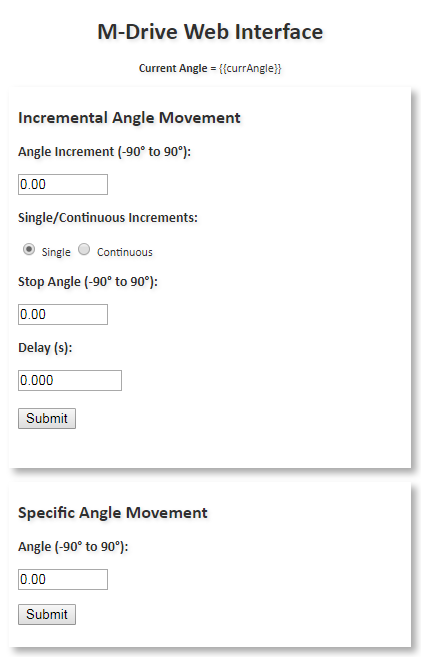
\includegraphics[scale=0.65]{img/m-drive_interface}
        \caption{HTML web interface for entering M-Drive motor commands}
        \label{fig:m-drive_interface}
    \end{figure}
    
    \subsection{Implementation} \label{m-drive_implementation}
    
    The server has been implemented in Python using an open-source server microframework called \texttt{Flask} \cite{flask}. The library enables the creation of locally hosted servers, and allows clients to transmit \texttt{HTTP} requests to the server, which uses Javascript to validate user data. To communicate with the M-Drive, the server uses the serial library \texttt{PySerial} \cite{pyserial}, which lets the server send a string of text to the M-Drive that is interpreted as different pre-defined movements. 
    
    A client of the server is able to tell the motor to move to a certain angle, or they can have it execute a relative movement of an incremental angle, either a single time or continuously until some stop angle is reached. A delay time between angle movements can also be set. Further documentation and source code can be found on the project's GitHub page \cite{m-drive_github}.

\section{Conclusion} \label{conclusion}

    Many of these projects are not completed to their fullest potential, and further work can always be done to test and improve their functionality. Hopefully this document clearly outlines the implementation of these projects for future student interns. Of course if anything is unclear, I can be contacted through Dr. Epp with any questions.
    
\pagebreak

\section{Appendix} \label{appendix}

    \subsection{Relevant File Locations}
    
    \begin{itemize}
        \item Public files from \texttt{Regaedat} computer - Including old Motionworks code, inherited files from previous interns
            \begin{verbatim}
    N:\regaedat\cfel
            \end{verbatim}
        \item Public files from Keenan - Including Motionworks and Arduino code, Data, MATLAB scripts, Documentation, SolidEdge parts and drawings
            \begin{verbatim}
    N:\mpsdgst5\cfel\Keenan_2018
            \end{verbatim}
        \item Public files from Pawel 
            \begin{verbatim}
    N:\mpsdgst9\cfel\Pavel_2018
            \end{verbatim}
    \end{itemize}
    
    \noindent\textbf{Note 1:} There may be some overlap between files found in these directories. 
    
    \noindent \textbf{Note 2:} The newest Arduino and MotionWorks code files should be named \texttt{BNCServer} and \texttt{CH1 07 12 2018 / CH2 07 12 2018} respectively
     
    \noindent \textbf{Note 3:} A backup of relevant files has also been put onto a USB stick, see Dr. Epp.
    
    \subsection{Operational Setup of Chopper System} \label{appendix_setup}
    
    \begin{figure}[h]
        \centering
        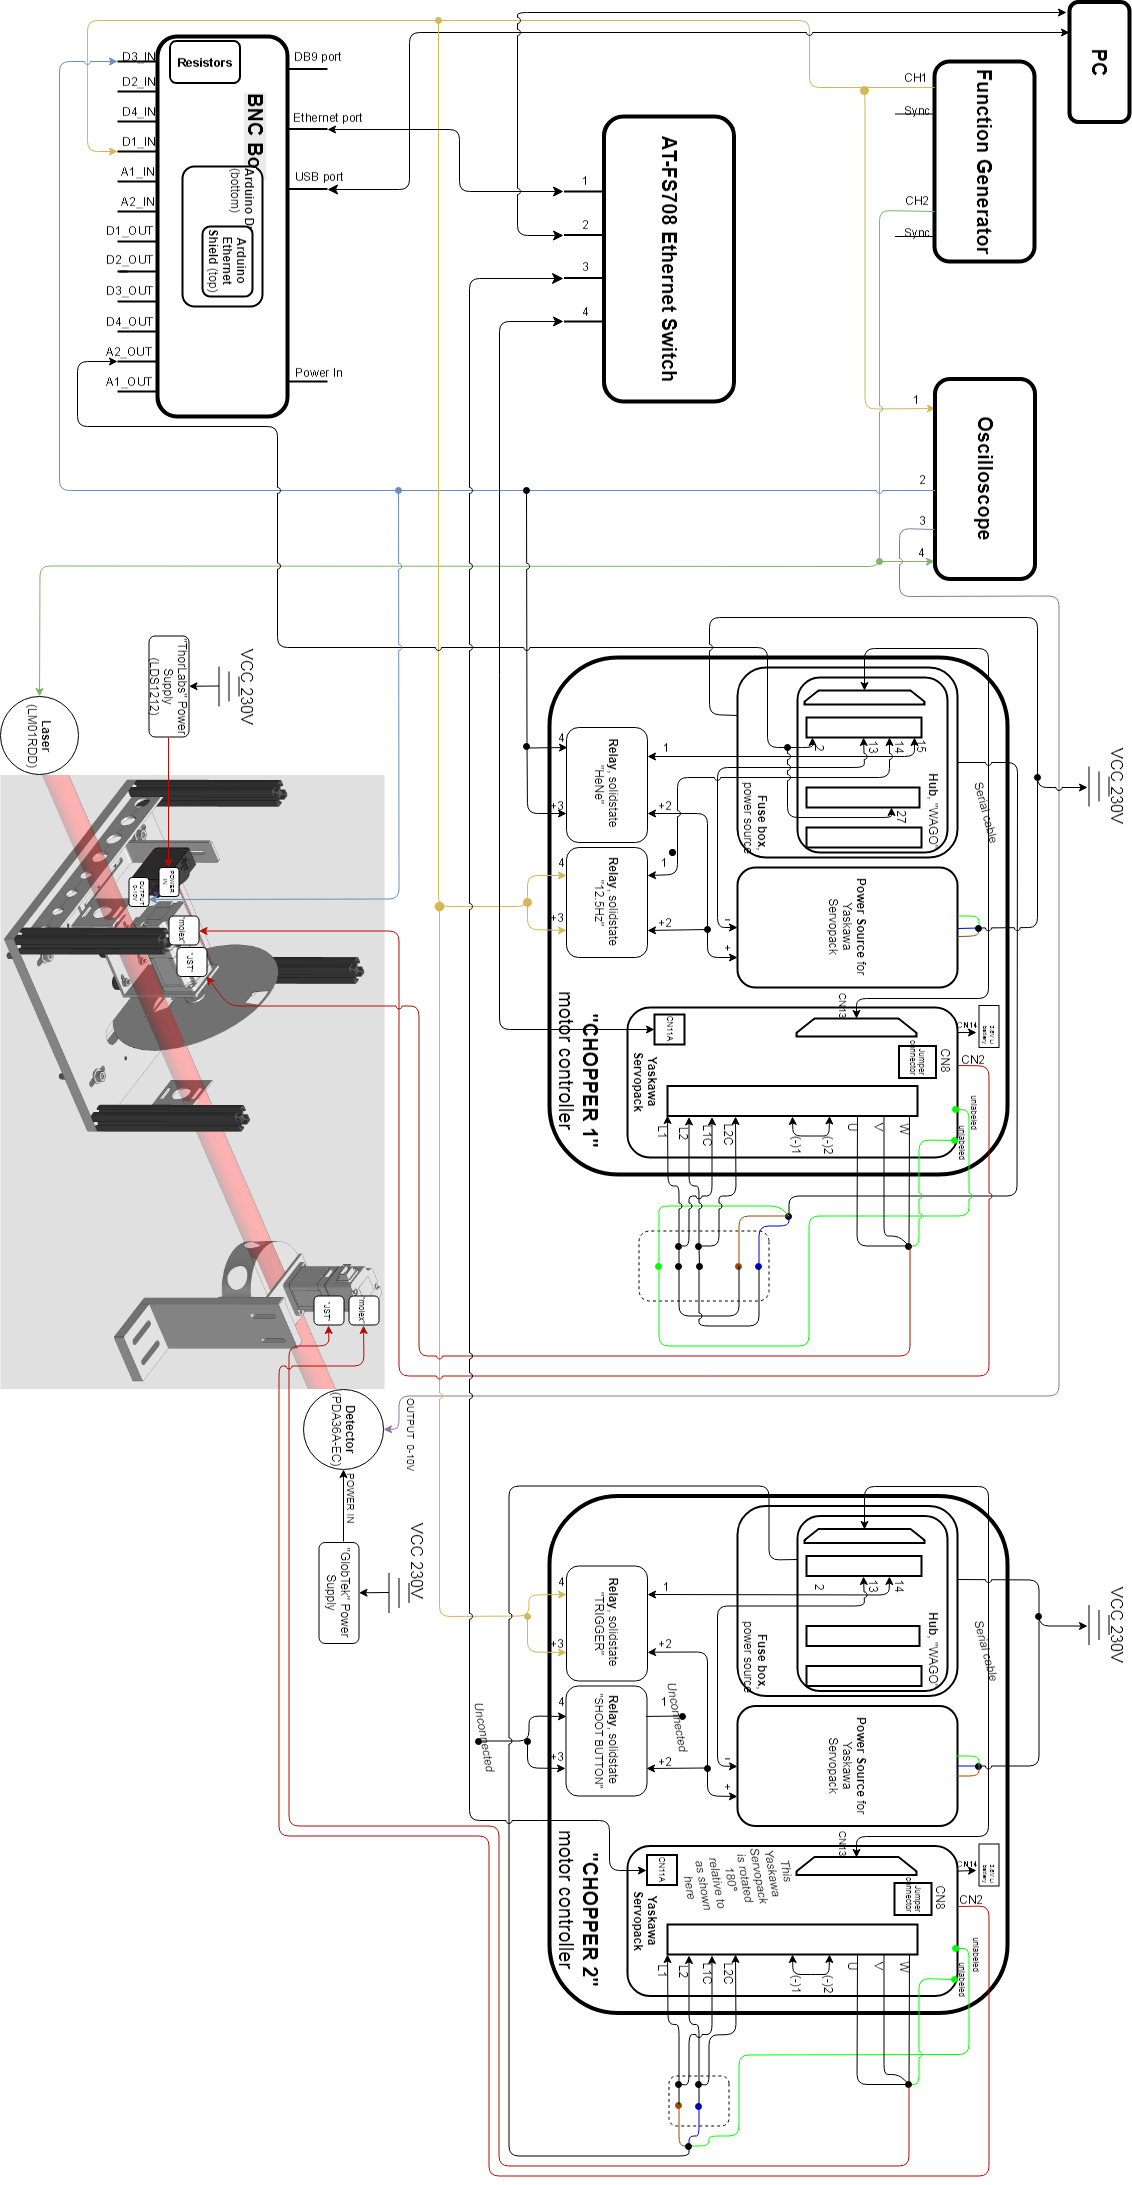
\includegraphics[scale=0.35]{img/chopper_setup_schematic}
        \caption{Full operational schematic of Chopper System}
        \label{fig:chopper_setup_schematic}
    \end{figure}
    
        \subsubsection{Function Generator Setup}
        
        \begin{enumerate}[label=\textbf{\arabic*}]
            \item Turn on the function generator
            \item Set Channel 1 to Generate a square-wave from 0 V to 5 V at 12.5 Hz, set to the smallest duty cycle
            \item Initially, make sure that the Channel Outputs of these functions are off
        \end{enumerate}
        
        \subsubsection{Arduino Due Box Setup}
        
        \begin{enumerate}[label=\textbf{\arabic*}]
            \item Turn on the Arduino Due by connecting a USB cable from a Windows computer (which has the Arduino interfacing tools installed on it) to the Arduino Due box
            \item Make sure that the \texttt{BNCServer.ino} Arduino Sketch has been uploaded onto the Arduino
            \item Ensure that an SD card with the correct file \texttt{regaedat.html} is loaded onto the Arduino
            \begin{itemize}
                \item It is possible to view all files on the SD card sending the \texttt{sd:print} command over serial connection
                \item The SD card must be formatted as \texttt{FAT16/FAT32}
            \end{itemize}
            \item Connect to the Arduino over serial USB with the correct settings: \texttt{Port = COM4} and \texttt{Baudrate = 9600}
            \begin{itemize}
                \item The Arduino IDE can be used or any other software for serial connections, for example PuTTy
            \end{itemize}
            \item By sending the serial command \texttt{vtt:?}, validate that the Arduino Due Box is set to the following configuration:
                \begin{enumerate}
                    \item \texttt{Max Time Delay = 20000(us)}
                    \item \texttt{Digital Input 1 = D3 IN}
                    \item \texttt{Digital Input 2 = D1 IN}
                    \item \texttt{Analog Output = A2 OUT}
                    \item \texttt{State: vtt2}
                    \item \texttt{LowerBound = 0}
                    \item \texttt{UpperBound = 4095}
                \end{enumerate}
            \item By sending the serial command \texttt{server:?}, verify that the Arduino's IP Address is set to \texttt{192.168.1.177} and port \texttt{80}
            \item Connect the 12.5 Hz Trigger signal from the function generator to the BNC port \texttt{D IN 1} on the Arduino Box
            \item Connect the HeNe Reference signal from the photodiode to the BNC port \texttt{D IN 3} on the Arduino Box
            \item When all the inputs are connected, begin the signal processing on the Arduino by sending the command \texttt{vtt:start:2CHAN}
            \item Connect the \texttt{A OUT 2} BNC port of the Arduino to the \texttt{VTT OUT} labelled BNC cable of Chopper 1.
        \end{enumerate}
        
        \subsubsection{Ethernet Connection Setup}
        
        \begin{enumerate}[label=\textbf{\arabic*}]
            \item Connect the Ethernet output of the Arduino BNC Box to the Ethernet Switch
            \item Connect an Ethernet port of any PC to the Ethernet Switch
            \item Make sure the IP Address of the PC’s Ethernet port is on the same local subnet of the 
            Arduino server, i.e. the first 3 bytes of the IP Address are the same as the Arduino’s (e.g.  \texttt{192.168.1.3})
            \item Connect Ethernet port CN11A of Chopper 1’s MP2600iec to the Ethernet Switch
            \item  Make sure the IP Address of this MP2600iec is set to \texttt{192.168.1.17} using the Hardware Config menu in MotionWorks software
            \begin{enumerate}
                \item To do this, the built-in E-INIT switch of the MP2600iec (found just above the large CN13 input port) must be set to OFF
                \item This allows a user to set a non-default IP Address
            \end{enumerate}
            \item Connect Ethernet port CN11A of Chopper 2's MP2600iec to the Ethernet Switch
            \item  Make sure the IP Address of this MP2600iec is set to \texttt{192.168.1.1} using the Hardware Config menu in MotionWorks software.
            \begin{enumerate}
                \item This should be the default IP Address of the Yaskawa
                \item You can force it to this default address by setting the built-in E-INIT switch of the controller to ON
            \end{enumerate}
            \item Open any browser on the PC, and connect to the IP Address of the Arduino Server, i.e.
            \texttt{192.168.177}
            \item You should now be able to send commands via browser to the Arduino by selecting a command and clicking the Submit button
        \end{enumerate}
        
        \subsubsection{Setup of Choppers 1 and 2}
        
        \begin{enumerate} [label=\textbf{\arabic*}]
            \item  Ensure connections are as shown in Figure 9 schematic
            \begin{enumerate}
                \item  Connect the 12.5 Hz signal from the function generator to the solid-state relay of Chopper 1 labelled as ”12.5 Hz”
            \end{enumerate}
            \item After all cables have been connected, there are 2 power sources that may need to be toggled for the motor controller
            \begin{enumerate}
                \item One for the solid-state relays, and one for the motor controller itself
                \item Pay careful attention when working with these power sources as they handle very high voltages
            \end{enumerate}
            \item The choppers should automatically find their homing positions even if they were moved while offline
            \item Upload the MotionWorks code onto the MP2600iec motor controllers as follows:
            \begin{enumerate}
                \item Turn on MotionWorks 2 software and open the latest project file
                \item Select Build - Rebuild Project
                \item Open the Project Control Dialog Box found in one of the top panels of the MotionWorks window
                \item On the Project Control Dialog Box, click the Download button
                \item On the Project Control Dialog Box, click the ’Warm’ Button to enable the project
                \item Repeat for other chopper
            \end{enumerate}
            \item Go to the function generator hardware and turn on the output of the 12.5 Hz and 1 kHz signals
             \item Connect to either Choppers by entering their IP address into any browser
            \begin{enumerate}
                \item For administrative access, the username is \texttt{Admin} and the password is \texttt{MP2600} (case sensitive)
                \item If the Choppers are not operating correctly, try rebooting through this menu
            \end{enumerate}
            \item You should now be able to send commands via browser to the Arduino by selecting a command and clicking the Submit button
            \begin{enumerate}
                \item You can observe live values of code variables in MotionWorks by clicking ’Debug On/Off’
                \item Logic Analyzer is also a very useful tool
                \item Both of these are explained in the Yaskawa online video training series
            \end{enumerate}
        \end{enumerate}
        
        \begin{figure}[h]
            \centering
            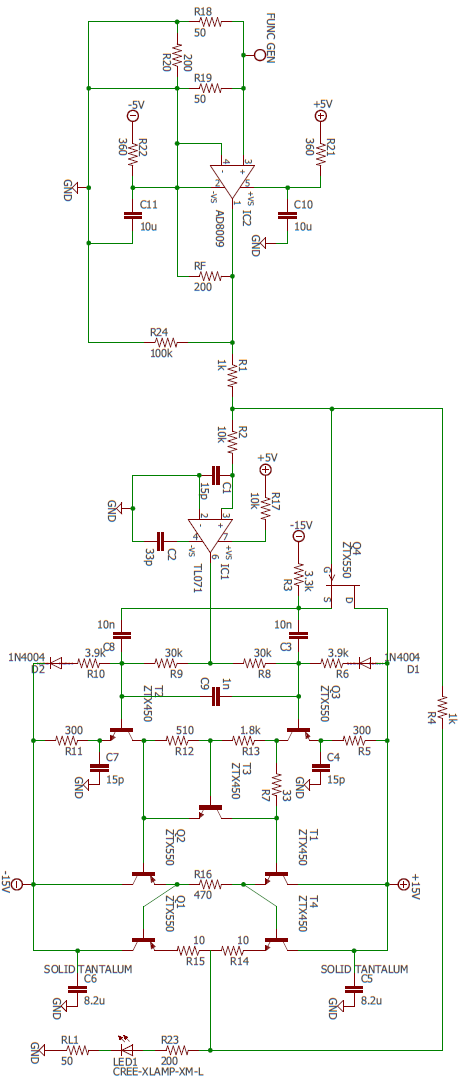
\includegraphics[scale=0.65]{img/nanosecond_led_circuit}
            \caption{Circuit to generate nanosecond-scale LED pulses}
            \label{fig:nanosecond_led_circuit}
        \end{figure}
    
        \begin{figure}[h]
            \centering
            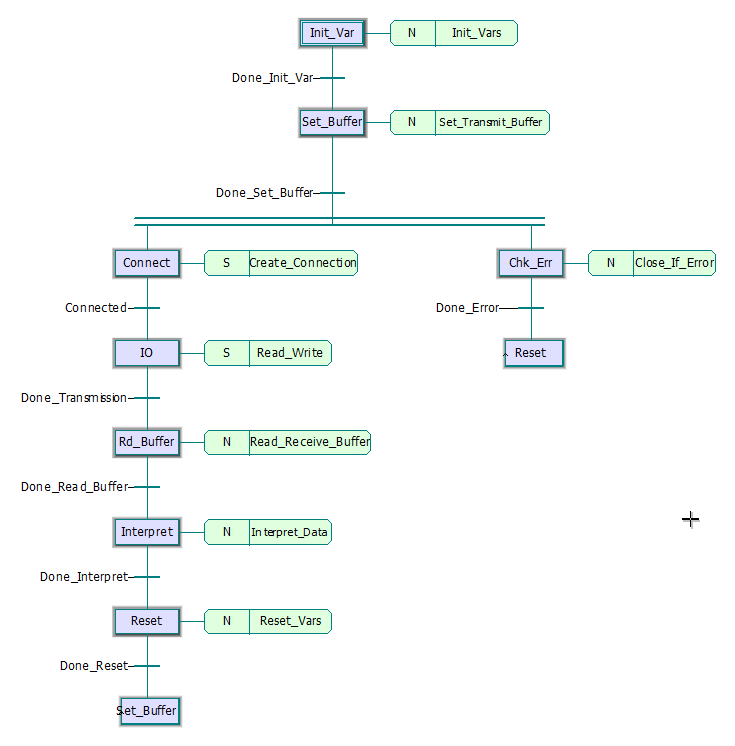
\includegraphics[scale=0.6]{img/ethernet_sfc}
            \caption{Ethernet IO SFC}
            \label{fig:ethernet_sfc}
        \end{figure}
        
        \begin{figure}[h]
            \centering
            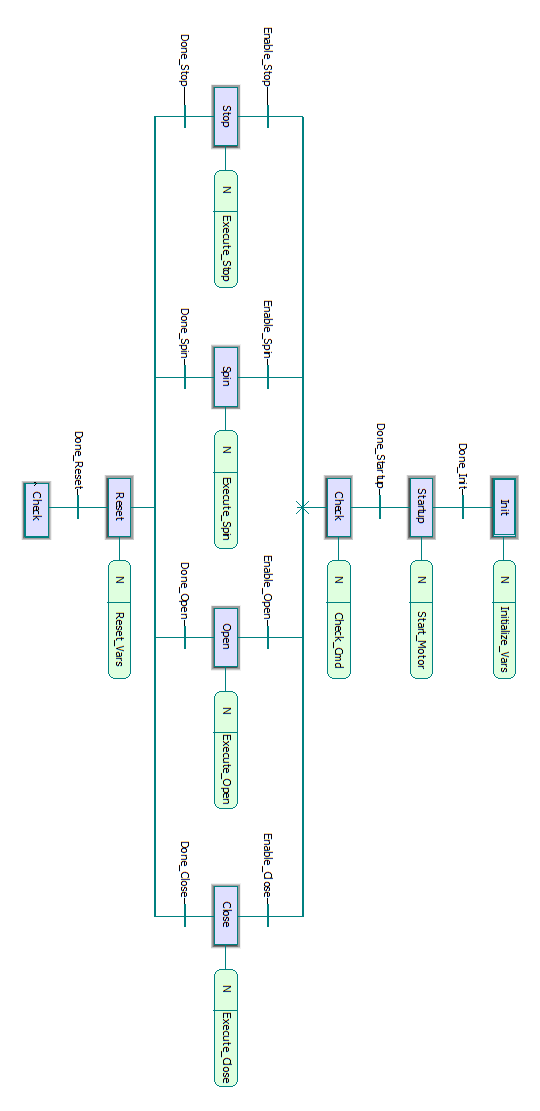
\includegraphics[scale=0.6]{img/ch1_sfc}
            \caption{Chopper 1 SFC}
            \label{fig:ch1_sfc}
        \end{figure}
        
        \begin{figure}[h]
            \centering
            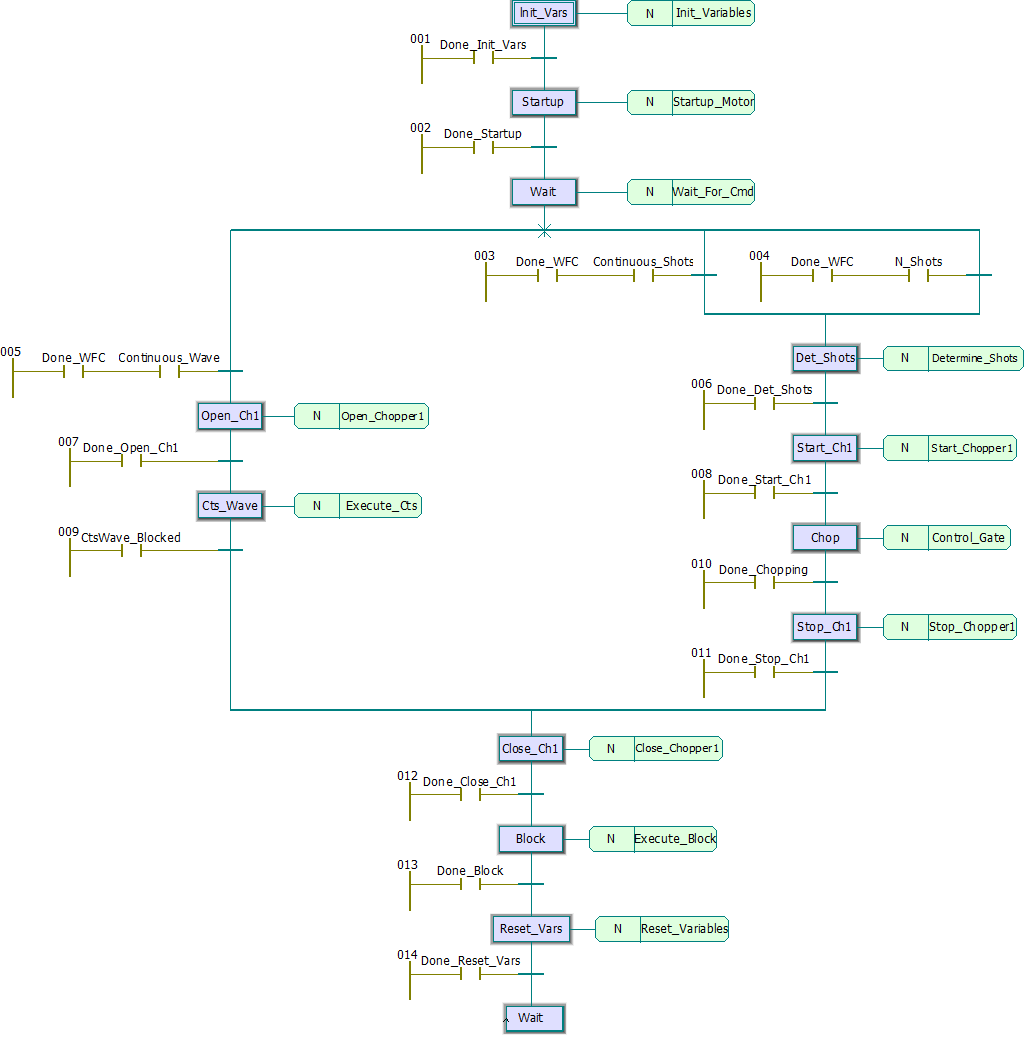
\includegraphics[scale=0.6]{img/ch2_sfc}
            \caption{Chopper 2 SFC}
            \label{fig:ch2_sfc}
        \end{figure}

\pagebreak

\bibliographystyle{IEEEtran}
\bibliography{IEEEabrv,references}

\end{document}
